\chapter{Implémentation}
\label{chaper-2}

Description fonctionnalités programme

Explication implémentation de l'algorithme de ray-tracing, et de la structure du code


\section{Interface utilisateur}
...

\begin{figure}[H]
    \centering
    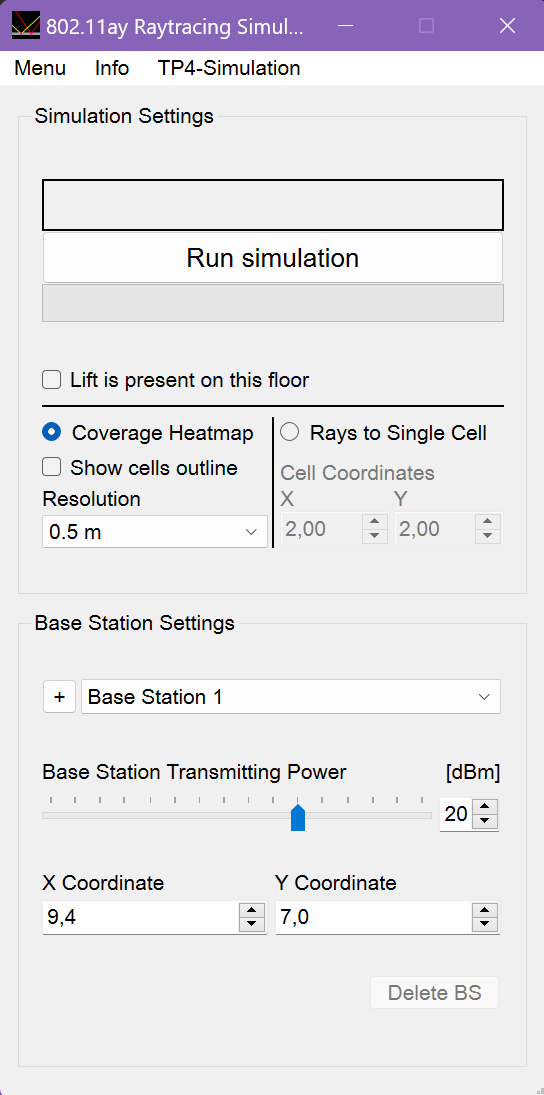
\includegraphics[width=0.5\textwidth]{latex/images/interface.png}
    \caption{Interface utilisateur du programme}
    \label{fig:interface}
\end{figure}

\section{Algorithme}
...

\section{Affichage}
...

\begin{figure}[H]
    \centering
    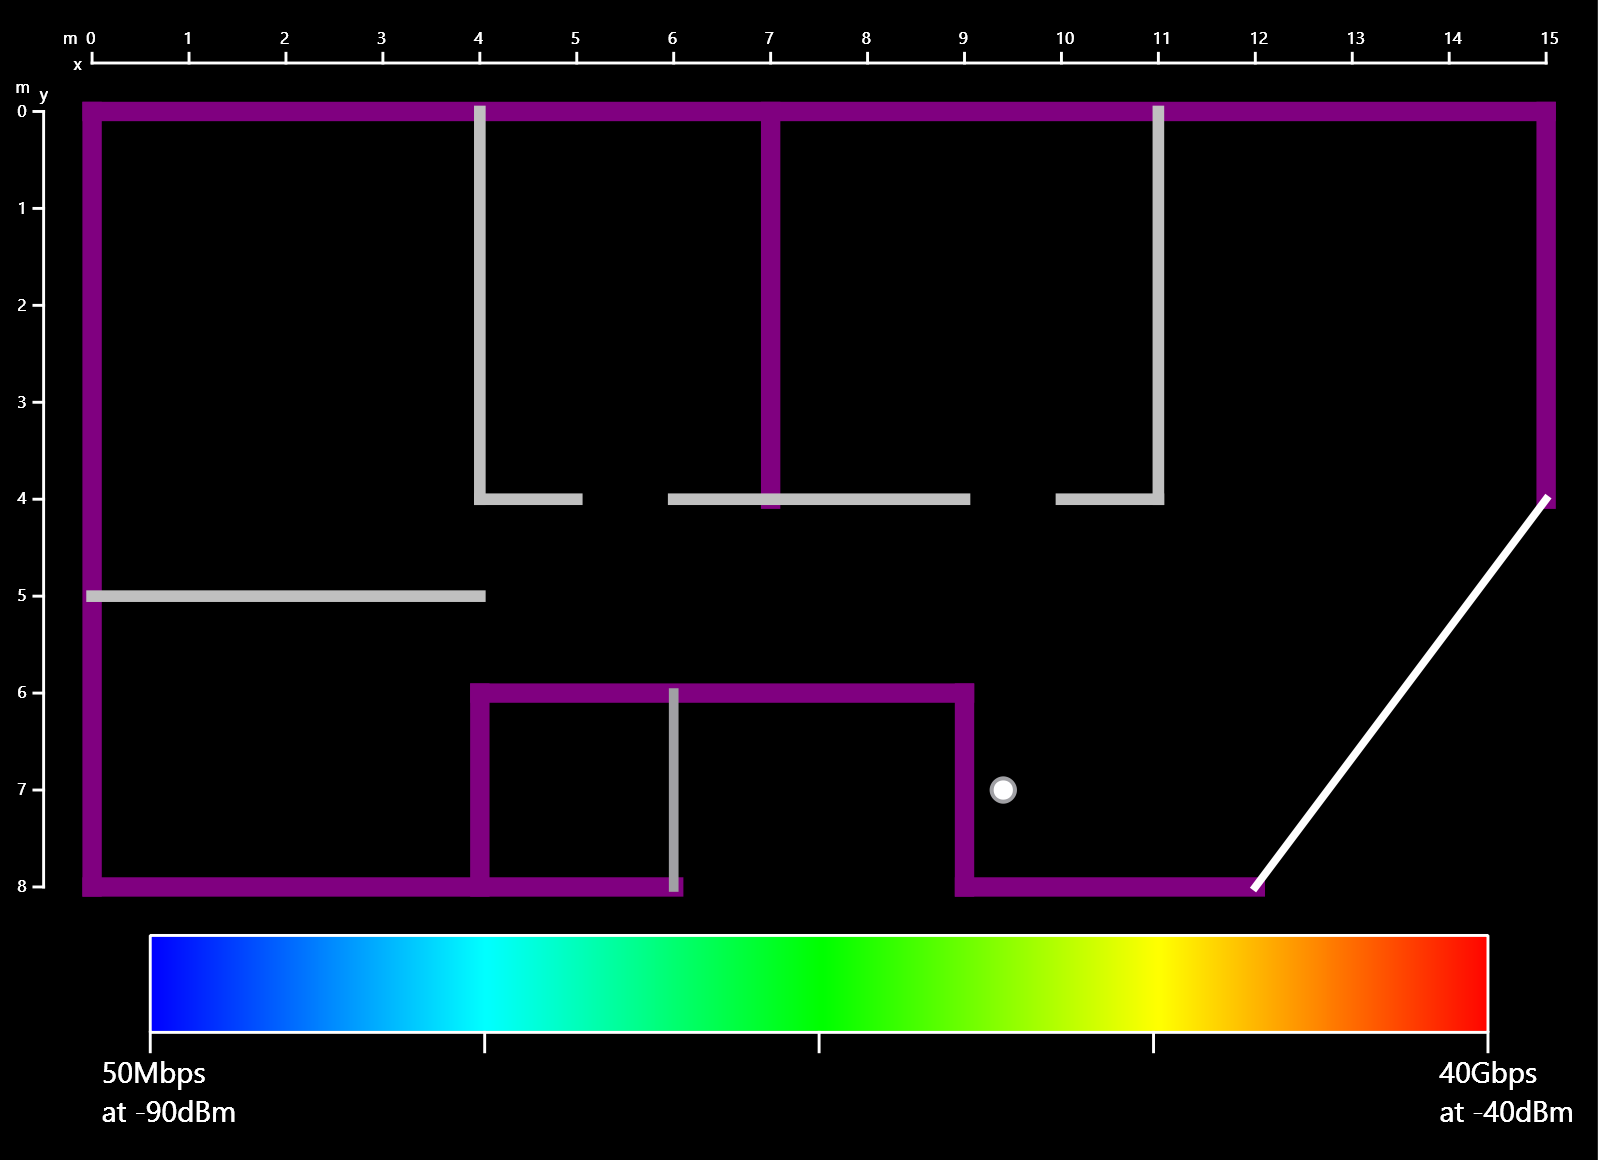
\includegraphics[width=\textwidth]{latex/images/blank_map.png}
    \caption{Carte vide de la simulation}
    \label{fig:blank-map}
\end{figure}

\section{Ajouts futurs possibles}
% décrire les futures ameliorations qui peuvent être ajoutées
...

\section{Performances}
% temps d'exécution, RAM etc
...

Le temps d'exécution pour une simulation exemple, de résolution de cellule de $0.125\mathrm{m}\times0.125\mathrm{m}$ est aux alentours des 500ms [Figure \ref{fig:time-0.125m}], soit des performances tout à fait acceptables.\\
Le temps d'exécution a été calculé grâce à un objet \mintinline{cpp}{QTimer}, lancé après une pression du bouton \textit{Run} et stoppé juste avant l'affichage graphique.
\begin{figure}[H]
    \centering
    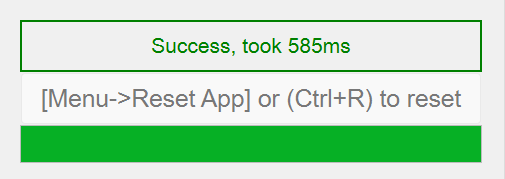
\includegraphics[width=0.7\textwidth]{latex/images/time-0.125m.png}
    \caption{Temps d'exécution simulation de résolution 0.125m}
    \label{fig:time-0.125m}
\end{figure}
